%!TEX program=lualatex
\documentclass[9pt,xcolor={dvipsnames},handout]{beamer}
\usetheme[
%%% options passed to the outer theme
    progressstyle=movCircCnt,   %either fixedCircCnt, movCircCnt, or corner
%    progressstyle=movCircCnt,   %either fixedCircCnt, movCircCnt, or corner
    rotationcw,          % change the rotation direction from counter-clockwise to clockwise
%    shownavsym          % show the navigation symbols
  ]{AAUsimple}
  
% \usepackage[utf8]{inputenc}
\usepackage[english]{babel}
\usepackage[T1]{fontenc}
\usepackage{epigraph}
\usepackage{amsmath}
% Or whatever. Note that the encoding and the font should match. If T1
% does not look nice, try deleting the line with the fontenc.
% \usepackage{helvet}

% colored hyperlinks
\newcommand{\chref}[2]{%
  \href{#1}{{\usebeamercolor[bg]{AAUsimple}#2}}%
}
\definecolor{colorAzulBienBonito}{RGB}{0,200,255}
\newcommand{\markdone}{\textcolor{PineGreen}{$\bullet$}}
\newcommand{\markonprogress}{\textcolor{colorAzulBienBonito}{$\bullet$}}
\newcommand{\markoff}{\textcolor{PineGreen}{$\circ$}}
\usepackage{booktabs}
\usepackage{makecell}
\usepackage{multicol}
\usepackage{multirow}

\usepackage{tikz}
\def\checkmark{\tikz\fill[scale=0.4](0,.35) -- (.25,0) -- (1,.7) -- (.25,.15) -- cycle;}
\usepackage{array}
\newcolumntype{L}[1]{>{\raggedright\let\newline\\\arraybackslash\hspace{0pt}}m{#1}}
\newcolumntype{C}[1]{>{\centering\let\newline\\\arraybackslash\hspace{0pt}}m{#1}}
\newcolumntype{R}[1]{>{\raggedleft\let\newline\\\arraybackslash\hspace{0pt}}m{#1}}



\usepackage{fontspec}
\setmainfont[]{Cardo} % sets the roman font
\setsansfont[]{PT Sans} % sets the sans font
\setmonofont[]{Consolas} % sets the monospace font

% %%%%% CHANGING THE FONT!
% \RequirePackage{etoolbox}
% % \RequirePackage{ifxetex}
% % \RequirePackage{ifluatex}
% \RequirePackage{pgfopts}

% \setsansfont[ItalicFont={Fira Sans Light Italic},%
%             BoldFont={Fira Sans},%
%             BoldItalicFont={Fira Sans Italic}]%
%             {Fira Sans Light}%
  
%       \setmonofont[BoldFont={Fira Mono Medium}]{Fira Mono}%

% \setbeamerfont{title}{size=\Large,%
%                       series=\bfseries}
% \setbeamerfont{author}{size=\small}
% \setbeamerfont{date}{size=\small}
% \setbeamerfont{section title}{size=\Large,%
%                               series=\bfseries}
% \setbeamerfont{block title}{size=\normalsize,%
%                             series=\bfseries}
% \setbeamerfont{block title alerted}{size=\normalsize,%
%                                     series=\bfseries}
% \setbeamerfont*{subtitle}{size=\large}
% \setbeamerfont{frametitle}{size=\large,%
%                            series=\bfseries}
% \setbeamerfont{caption}{size=\small}
% \setbeamerfont{caption name}{series=\bfseries}
% \setbeamerfont{description item}{series=\bfseries}
% \setbeamerfont{page number in head/foot}{size=\scriptsize}
% \setbeamerfont{bibliography entry author}{size=\normalsize,%
%                                           series=\normalfont}
% \setbeamerfont{bibliography entry title}{size=\normalsize,%
%                                          series=\bfseries}
% \setbeamerfont{bibliography entry location}{size=\normalsize,%
%                                             series=\normalfont}
% \setbeamerfont{bibliography entry note}{size=\small,%
%                                         series=\normalfont}
% \setbeamerfont{standout}{size=\Large,%
% series=\bfseries}
% %%%%%%%%%%%%%%%%%%%%%%%%%%%%

\title[Smart usage of context information for the analysis, design and generation of power-aware policies for MSA's]{Smart usage of context information for the analysis, design and generation of power-aware policies for mobile sensing apps}
         
\date{Doctoral seminar 2016}
\author{
  Rafael Pérez Torres
}

\institute[
  ITL Information Technology Laboratory\\
  Cinvestav\\
  Tamaulipas
] 
{  Dr. César Torres Huitzil\\
  Dr. Hiram Galeana Zapién\\

  LTI Cinvestav
  
}

% specify a logo on the titlepage (you can specify additional logos an include them in 
% institute command below
\pgfdeclareimage[height=1.5cm]{titlepagelogo}{AAUgraphics/aau_logo_new} % placed on the title page
%\pgfdeclareimage[height=1.5cm]{titlepagelogo2}{AAUgraphics/aau_logo_new} % placed on the title page
\titlegraphic{% is placed on the bottom of the title page
  \pgfuseimage{titlepagelogo}
%  \hspace{1cm}\pgfuseimage{titlepagelogo2}
}

\graphicspath{{../../../resources/images/}}
\begin{document}
% the titlepage
{\aauwavesbg%
\begin{frame}[plain,noframenumbering] % the plain option removes the header from the title page
  \titlepage
\end{frame}}
%%%%%%%%%%%%%%%%

% TOC
\begin{frame}{Agenda}{}
\tableofcontents
\end{frame}
%%%%%%%%%%%%%%%%

\section{Background}
\begin{frame}{Background}{Motivation}
\begin{itemize}
  \item<1-> The popularity of mobile devices is a result of advances in their computation, \textbf{sensing}, and communication dimensions~\cite{Islam2014}.
  \begin{itemize}
    \item<1-> The sensing facilities improve interaction with user, turning them into \emph{omni-sensors} able to \emph{know} about its surrounding environment.
    \item<2-> Smartphones have become \emph{context-aware} devices, gaining understanding about user's activity and environment.
    \item<3-> \textbf{Context} is the set of environmental states and settings that either determines an application's behavior or in which an application event occurs and is interesting to the user~\cite{Chen2000}.
  \end{itemize}
  \item<4-> However, battery is not evolving at the same pace of advances in other smartphone's characteristics~\cite{Kjaergaard2012}, growing only 5-10\% each year~\cite{Ma2012,Evarts2015}.
  \begin{itemize}
    \item The energy constraint becomes critical when continuous access to sensors is needed, which is a core requirement of \textbf{mobile sensing applications}. 
  \end{itemize}
\end{itemize}
\end{frame}

\section{Problem statement}
\begin{frame}{Problem definition}{Overall problem identification}
\begin{exampleblock}{Overall issue}
Conceptually, the main problem pursued by this research work is to design a location provider aware of the energy limitations of the mobile device.
Nonetheless, as the location is a reflection of the mobility patterns described by people, a set of more specific problems could be addressed.
\end{exampleblock}

\begin{exampleblock}{Types of mobility patterns}
There are two types of mobility patterns considered by this research:
\begin{itemize}
  \item Fine grain mobility patterns.
  \item Coarse grain mobility patterns.
\end{itemize}
\end{exampleblock}
\end{frame}

\begin{frame}{Problem definition}{Problem statement}
\begin{alertblock}{Problem 1: Mobility pattern identification}
Given a set of values $\mathcal{V} = v_1,v_2,\ldots,v_n$ obtained from sensor $\mathcal{S}$ in time range $[t_1,t_2]$, identify coarse-grain or fine-grain mobility information:
$$
\text{PatternIdentifier}(\mathcal{V}) \rightarrow p_S \in \text{Patterns}
$$
where Patterns  $ = \{ \text{static, walking, running, vehicle} \}$ for fine-grain location information, while for coarse-grain information refers to the arrival and departure to-from stay points described by user's mobility.

Additionally, the sensor $\mathcal{S}$ for fine-grain information is \texttt{accelerometer}, while sensor $\mathcal{S}$ for coarse-grain information is \texttt{GPS}.
\begin{figure}[tb]
  \centering
  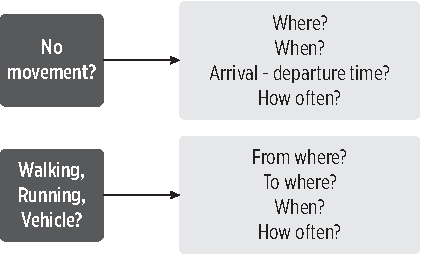
\includegraphics[scale=0.5]{vectors/mobility-patterns-implications}
  \caption{Context information related to mobility patterns}
  \label{fig:mobility-patterns-implications}
\end{figure}
\end{alertblock}
\end{frame}

\begin{frame}{Problem definition}{Problem statement}
\begin{alertblock}{Problem 2: Policy generation}
Given the set of detected mobility patterns $\mathcal{P} = \{ p_{S_1}, p_{S_2}, \ldots, p_{S_n} \}$ in data from sensors $\mathcal{S} = \{ S_1,S_2,\ldots, S_n \}$, accuracy required $a$, and physical constraints status $c$ of a mobile device, find a policy that select the proper set of sensors $\mathcal{S}_{new}$ and its associated configuration $\mathcal{S}_{new_{conf}}$  while meeting application requirements.

\begin{equation}
  \text{PolicyGeneration}( \mathcal{P}, a, c ) \longrightarrow{} \mathcal{S}_{new}, \mathcal{S}_{new_{conf}}
\end{equation}

The $\mathcal{S}_{new_{conf}}$ configuration is referred to as the \emph{adaptive duty cycle} of associated sensors.
\end{alertblock}
\end{frame}

\begin{frame}{Problem definition}{Interaction between problems}
\begin{figure}[tb]
  \centering
  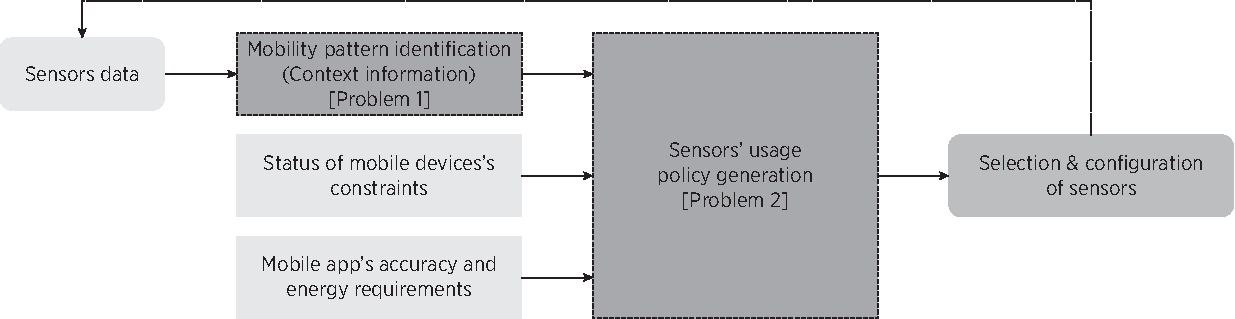
\includegraphics[width=\textwidth]{../../../resources/images/vectors/problems-incorporation}
  \caption{Interaction between problems}
  \label{fig:problems-incorporation}
\end{figure}
\end{frame}

\begin{frame}{Problem definition}{Hypothesis}
\begin{exampleblock}{Hypothesis}
Dynamic policies driven by events detected in user mobility could reduce energy consumption of the mobile device when performing continuous location tracking.
User mobility could be expressed by means of a spatial-time model learned from short and long time windows of context information extracted from GPS and accelerometer sensors data.
\end{exampleblock}
%\pause
{
\small
\pause
\begin{itemize}
  \item An intelligent policy is a special rule that defines how sensors should be selected and configured to reduce energy consumption and achieve the mobile sensing app's requirements.
  It is intelligent in terms of self-adaptness to changes detected in context information across time.
  \pause
  \item This research work is aimed at employing GPS and inertial sensors data (accelerometer) for inferring context information in terms of mobility patterns.
  This context information will then be exploited to adapt sensors' operation and produce power savings.
\end{itemize}
}
\end{frame}

\begin{frame}{Problem definition}{Objectives}
\begin{exampleblock}{Main objective}
To reduce energy consumption in the mobile sensing apps, which perform continuous sensor readings, through self-adapting power-aware policies generated from context information obtained from sensors data.
\end{exampleblock}
\pause

\begin{exampleblock}{Particular objectives}
\begin{itemize}
  \item To identify mobility patterns from context information obtained from an inertial sensor (accelerometer) and location providers (GPS).
  \pause
  \item To generate an accurate representation of mobility patterns, which in conjunction with accuracy mobile app requirements and mobile device constraints, allows to create power-aware GPS sensing policies.
  \pause
  \item To reduce energy consumption in location-based mobile sensing apps through a middleware that implements policies fed with mobility patterns learned from sensors data. 
  The middleware also eases the development of LBS, isolating the complexity of energy efficient sensors management.
\end{itemize}
\end{exampleblock}
\end{frame}

\begin{frame}{Problem definition}{Expected contributions}
\begin{itemize}
  \item<+-> A mechanism for detecting mobility patterns from the data read by sensors of mobile devices (GPS and accelerometer).
  \item<+-> A mechanism for generating policies for accessing sensors.
  The produced policies will allow to perform an intelligent usage of smartphone's sensing facilities in continuous sensor sampling, reducing the energy consumption.
  \item<+-> A middleware implementing the previous power-aware mechanisms for easing the development of location based services.
\end{itemize}
\end{frame}

\section{Methodology}
\begin{frame}{Methodology}{Methodology steps}
\begin{enumerate}
  \item \textbf{Familiarization with state-of-art power-aware sensing related techniques}
  \item \textbf{Formal definition and selection of mobility patterns to be identified}
  \item \textbf{Research on pattern recognition algorithms focused on mobility patterns identification}
  \item \textbf{Design of the Pattern Identification Element (PIE)}
  \item \textbf{Research on (and proposition of) adaptive policies for energy efficient usage of sensors}
  \item \textbf{Design of the Policy Generation Element (PGE)}
  \item Development of a middleware involving the PIE and PGE for the Android platform
  \item Experimentation in terms of accuracy and energy efficiency
\end{enumerate}
\end{frame}

\section{Related work}
\begin{frame}{Related work}{Previous work}
\begin{figure}
  \centering
  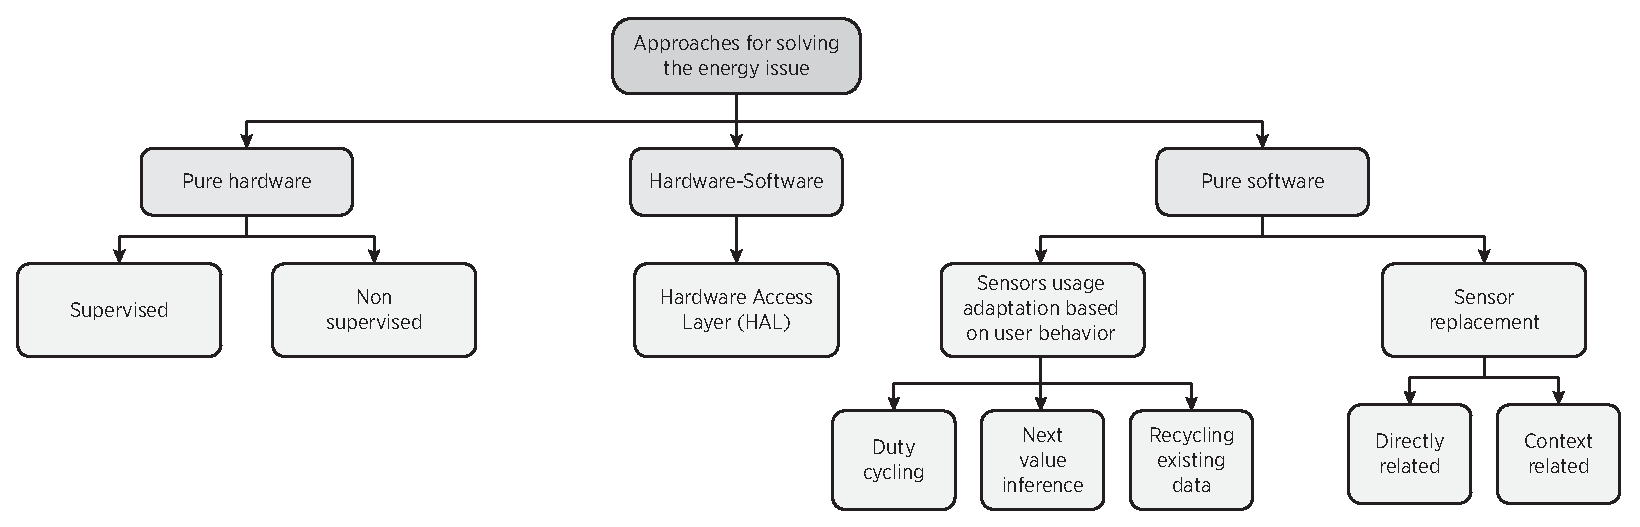
\includegraphics[width=\textwidth]{../../../resources/images/vectors/approaches-taxonomy}
  \caption{Taxonomy of related work solutions}
  \label{fig:taxonomy}
\end{figure}
\end{frame}

\begin{frame}{Related work}{Pure hardware approach}
\begin{exampleblock}{Pure hardware approach}
\begin{itemize}
  \item The fundamental idea is the selection of power-aware hardware elements for providing physical data to upper layers, as well as the definition of mechanisms to adapt the hardware input parameters, like DVFS\footnote{DVFS, Dynamic Voltage and Frequency Scaling}.
  \item Such mechanisms define control points for manipulating hardware (also known as power modes~\cite{Ranganathan2010,Lorch1998,Benini2000}).
  \item The hardware components obey a static behavior defined by power modes, whose control points are exported to upper layers of the mobile platform.
\end{itemize}
\end{exampleblock}

\begin{exampleblock}{Variants}
\begin{itemize}
  \item Ad-hoc data acquisition
  \item Co-processing
\end{itemize}
\end{exampleblock}
\end{frame}

\begin{frame}{Related work}{Hardware-software approach}
\begin{exampleblock}{Hardware-software approach}
\begin{itemize}
  \item It is aimed at defining system-wide policies for deciding when to turn sensors on and off, or when to switch hardware components to a different power mode.
  \item It abstracts fine-grain operation parameters into a coarse-grain set, easing the hardware usage for upper platform layers.
  \item It is also able to detect changes in the workload of hardware components.
  \item Because of the coupled interaction with hardware, solutions are produced as HAL's, or low-level hardware middlewares.
\end{itemize}
\end{exampleblock}
\end{frame}

\begin{frame}{Related work}{Pure software approach}
\begin{exampleblock}{Pure software approach}
\begin{itemize}
  \item \emph{Spending power to save power}~\cite{Ranganathan2010}.
  \item It employs context information obtained from sensor data, for achieving activity awareness and making informed decisions towards dynamic power-aware sensors management.
  \item The lower layers know how to turn circuits on and off, but are unable to define when; whereas higher software layers can dynamically adapt to changes in user context, delegating how to do it to the lower layers.
  \item Typically, pure software approach solutions are implemented through a layered middleware with the classification and machine learning modules embedded on it.
\end{itemize}
\end{exampleblock}
\end{frame}

\begin{frame}{Related work}{Pure software approach}
\begin{multicols}{2}
\begin{exampleblock}{Variants}
\begin{itemize}
  \item Sensors usage adaptation
    \begin{itemize}
      \item Duty cycling
      \item Next value inference
      \item Recycling existing data
    \end{itemize}
  \item Sensors replacement
  \begin{itemize}
    \item Directly related
    \item Context related
  \end{itemize}
\end{itemize}
\end{exampleblock}

\newpage
{\small Generic pure software approach middleware}
  {
  \centering
  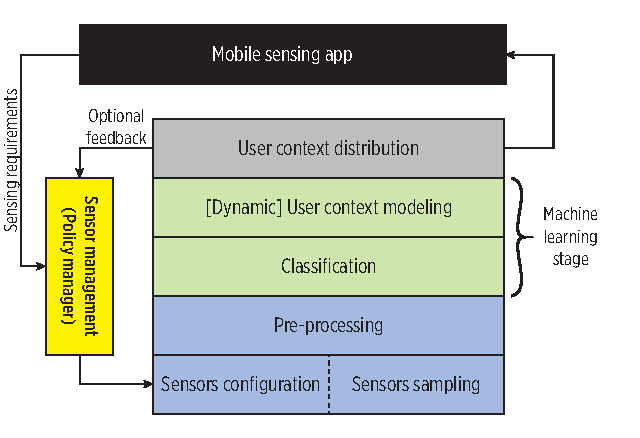
\includegraphics[width=1.2\columnwidth]{vectors/generic-middleware-architecture-v2}
  }
\end{multicols}
\end{frame}


\begin{frame}{Related work}{Characteristics of pure software approach solutions}
\begin{exampleblock}{Distinctive characteristics of pure software approach solutions}
\begin{itemize}
  \item \textbf{Optimization oriented (OO)}: Optimization orientation focused on minimizing energy consumption and/or the error in activity tracking.
  \item \textbf{Online learning (OL)}: Online learning from context information, enabling predictive features thanks to observance over long-time windows of sensory data.
  \item \textbf{User state oriented (US)}: Modeling of an enriched version of the context information, user state (US), for achieving full activity-awareness and ease the adaptation over the sensing dimension.
\end{itemize}
\end{exampleblock}
\end{frame}

\section{Solution}
\begin{frame}{Proposed solution}{Problem's scenario}
\begin{figure}
  \centering
  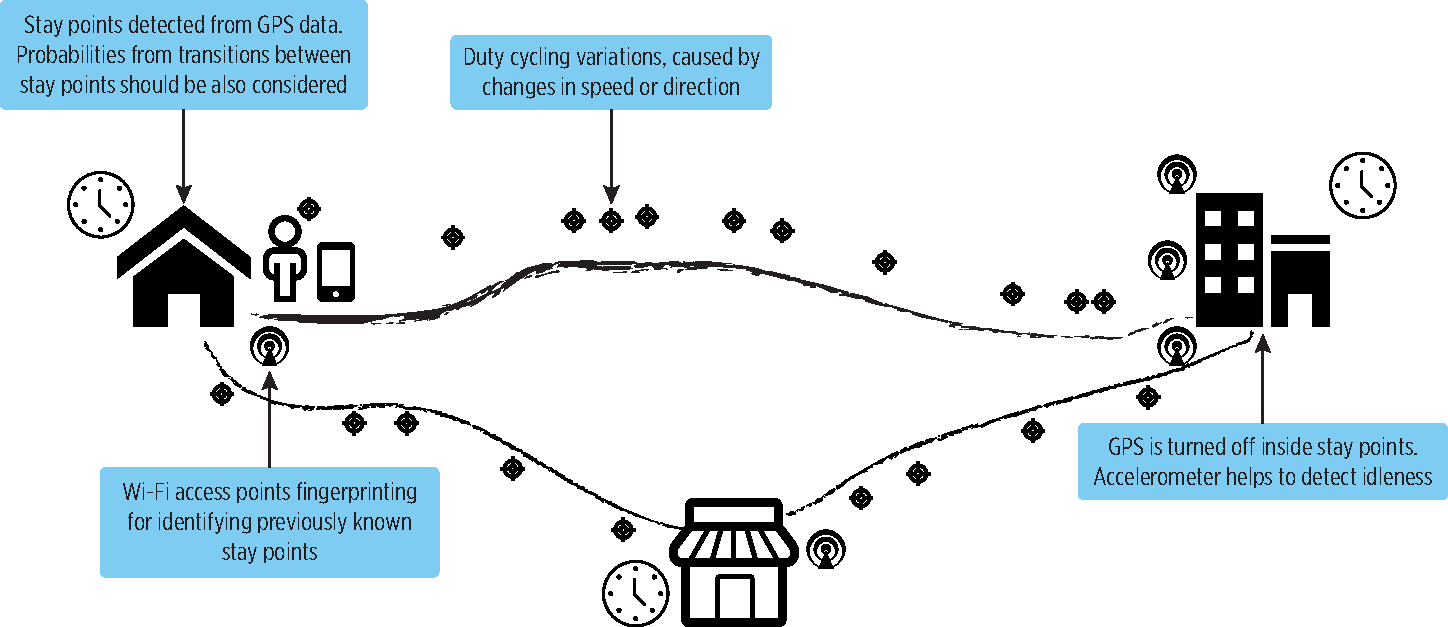
\includegraphics[width=\textwidth]{vectors/scenario}
  \caption{Basic problem's scenario}
  \label{fig:scenario}
\end{figure}
\end{frame}

\begin{frame}{Proposed solution}{Characteristics}
\begin{itemize}
  \item Pure software approach, implementing all of its variations.
  \pause
  \item Online learning and user state oriented.
  \pause
  \item Event-driven oriented, completely on device.
  \begin{itemize}
    \item Top level mobility states-events: \texttt{on trajectory}, \texttt{on stay point}.
    \pause
    \item Low level mobility states-events: \texttt{transportation mode changed}, \texttt{arriving to stay point}, \texttt{leaving stay point}.
    \pause
  \end{itemize}
  \item Inspired on Cognitive Dynamic Systems~\cite{Haykin2006}, including 
  \begin{itemize}
    \item Perception-action cycle.
    \pause
    \item Memory.
    \pause
    \item Attention.
    \pause
    \item Intelligence.
  \end{itemize}
\end{itemize}
\end{frame}

\begin{frame}{Proposed solution}{Overview}
\begin{figure}
  \centering
  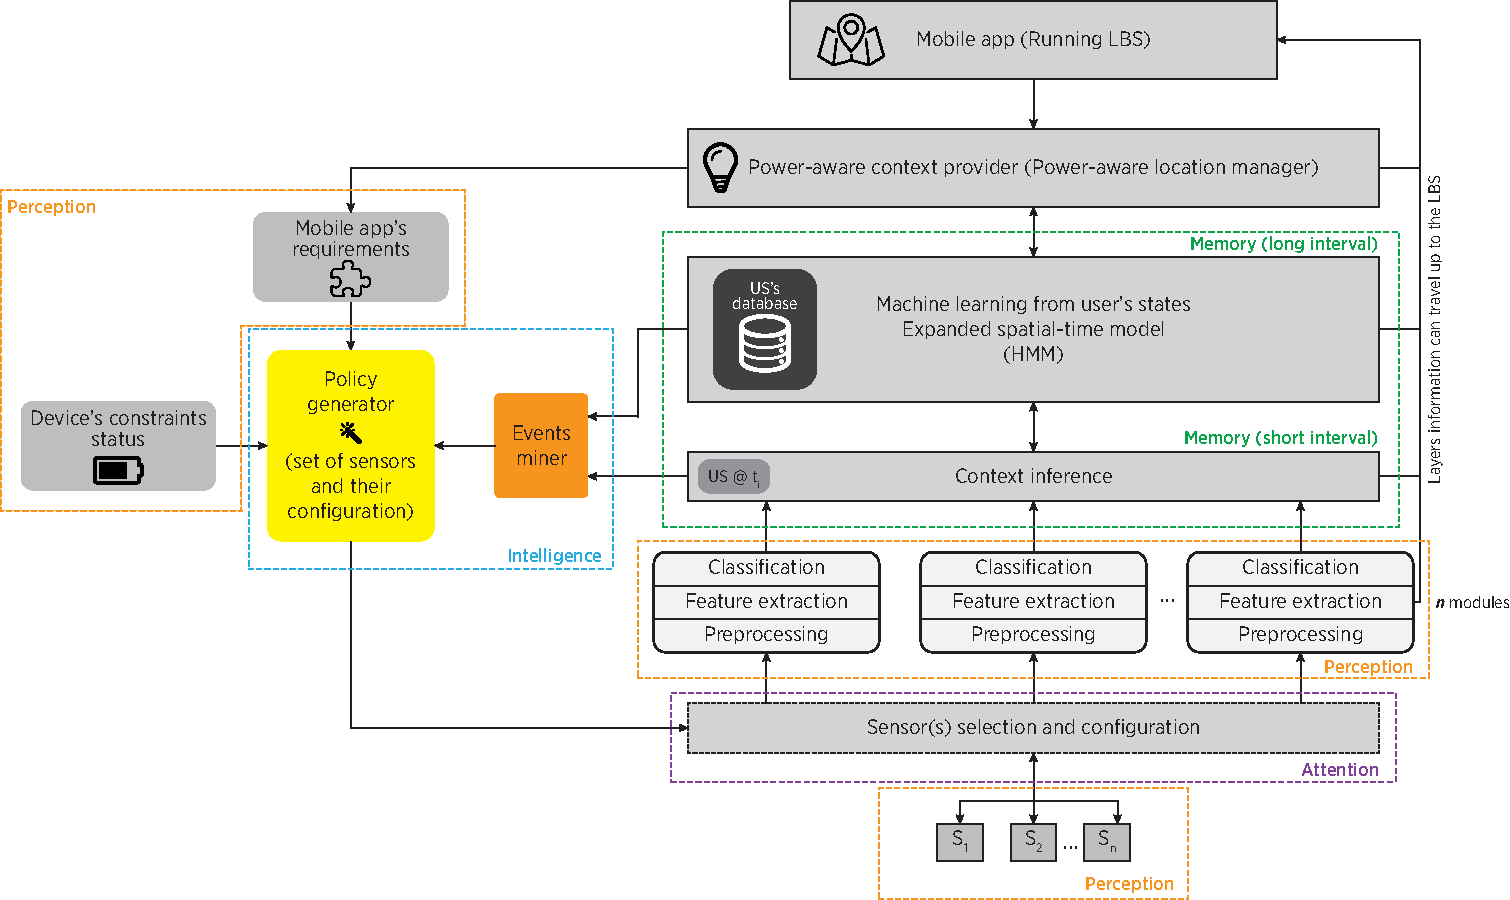
\includegraphics[width=\textwidth]{vectors/solution-general-overview}
  \caption{The layers of proposed solution}
  \label{fig:solution}
\end{figure}
\end{frame}

\begin{frame}{Proposed solution}{Operation}
\begin{itemize}
  \item Overall problem divided in:
  \begin{itemize}
    \item Detection and learning of stay points (The anchor points that user visits frequently).
    \pause
    \item Tracking of user commuting between stay points (Transition probability).
  \end{itemize}
\end{itemize}
\pause
\begin{figure}
  \centering
  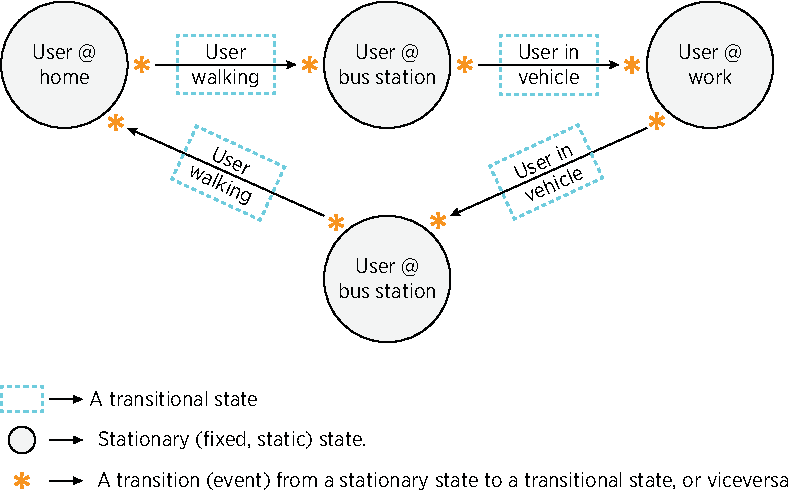
\includegraphics[width=0.55\textwidth]{vectors/zoom-expanded-spatial-time-model}
  \caption{Information modeled by the expanded spatial-time model}
  \label{fig:information-modeled-spatial-time-model}
\end{figure}
\end{frame}

\begin{frame}{Proposed solution}{Event-driven implementation}
\begin{figure}
  \centering
  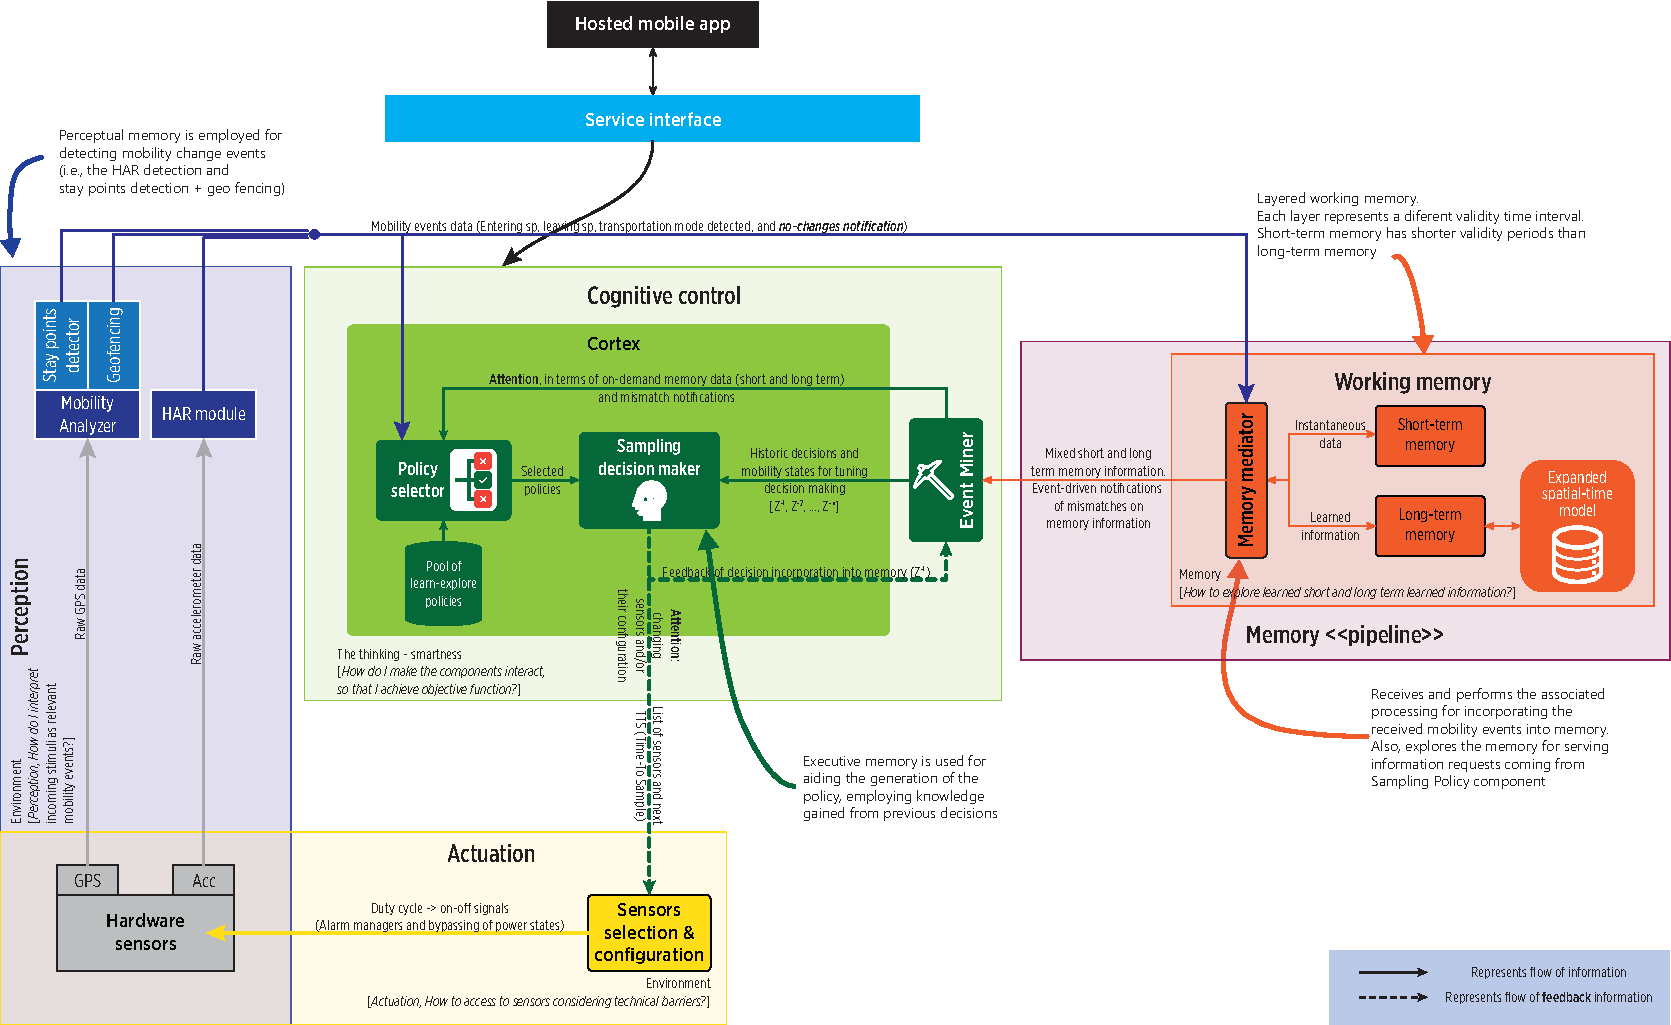
\includegraphics[width=1\textwidth]{vectors/smartness-components-v4}
  \caption{Cognitive components of platform and their interaction}
  \label{fig:cognitive-components}
\end{figure}
\end{frame}

\section{Preliminary results}
\begin{frame}{Preliminary results}{Feasibility of on-device mobility analysis}
% \begin{exampleblock}{Feasibility of on-device mobility analysis}
{
  \small{}
\begin{itemize}
  \item Several experiments were carried out for exploring the feasibility of performing on-device mobility analysis.
  \item Feasibility is understood as the ability for executing the middleware in the mobile device~\footnote{\scriptsize Google Nexus 6, 2.7 GHz quad-core processor, 3 GB RAM, 3220 mAh battery, Android 6.} under different stress levels without a premature finalization caused by CPU and memory consumption usage issues.
\end{itemize}
}
% \end{exampleblock}

\begin{table}
\centering
\caption{Summary of results of first experiment (SP = stay point).}
\label{tbl:experiment-1}
\resizebox{0.68\textwidth}{!}{%
\begin{tabular}{@{}ccccc@{}}
\toprule
\textbf{\begin{tabular}[c]{@{}c@{}}Sampling\\ period  (seconds)\end{tabular}} & \textbf{\begin{tabular}[c]{@{}c@{}}Event-driven\\ algorithm\end{tabular}} & \textbf{\begin{tabular}[c]{@{}c@{}}Obtained\\ GPS fixes\end{tabular}} & \textbf{\begin{tabular}[c]{@{}c@{}}Average GPS\\ fixes per SP\end{tabular}} & \textbf{\begin{tabular}[c]{@{}c@{}}Running time \\ (minutes)\end{tabular}} \\ \midrule
\multirow{2}{*}{30 seconds} & Buffered & 3,876 & 218.3 & 6,752 \\
 & Sigma & 5,199 & 244.4 & 8,243 \\
 \cmidrule{2-5}

\multirow{2}{*}{60 seconds} & Buffered & 5,307 & 155.6 & 14,877 \\
 & Sigma & 3,054 & 126.3 & 8,428 \\
 \cmidrule{2-5}

\multirow{2}{*}{90 seconds} & Buffered & 2,573 & 115.2 & 7,694 \\
 & Sigma & 2,447 & 108.1 & 7,522 \\
 \cmidrule{2-5}

\multirow{2}{*}{120 seconds} & Buffered & 1,708 & 77.4 & 8,460 \\
 & Sigma & 1,993 & 82.2 & 10,214 \\
 \cmidrule{2-5}

\multirow{2}{*}{150 seconds} & Buffered & 1,417 & 53.8 & 10,433 \\
 & Sigma & 1,651 & 51.1 & 10,349 \\
 \bottomrule
\end{tabular}%
}
\end{table}
\end{frame}


\begin{frame}{Preliminary results}{Energy performance (solution vs MCC oriented approach)}
{
\small{}
\begin{itemize}
  \item Purpose of comparing the energy consumption of the proposed middleware with respect to an MCC oriented solution that offloads location data processing.
  \item The MCC oriented solution subscribed for location updates to the middleware, but translated each location update into a string representation (116 bytes, in average) sent to an application server using cellular data network.
\end{itemize}
}

\begin{table}
\centering
\resizebox{\textwidth}{!}{%
\begin{tabular}{@{}cccccccc@{}}
\toprule
\textbf{\begin{tabular}[c]{@{}c@{}}Sampling\\period\\(seconds)\end{tabular}}  & \textbf{\begin{tabular}[c]{@{}c@{}}Processing\\ strategy\end{tabular}} & \textbf{\begin{tabular}[c]{@{}c@{}}Obtained \\ GPS fixes\end{tabular}} & \textbf{\begin{tabular}[c]{@{}c@{}}GPS-on time\\ (minutes)\end{tabular}} & \textbf{\begin{tabular}[c]{@{}c@{}}Average \\ acquisition \\  time per fix\\ (seconds)\end{tabular}} & \textbf{\begin{tabular}[c]{@{}c@{}}Running time\\ (minutes)\end{tabular}} & \textbf{\begin{tabular}[c]{@{}c@{}}Data sent\\ (bytes)\end{tabular}} & \textbf{\begin{tabular}[c]{@{}c@{}}Data received\\ (bytes)\end{tabular}} \\ \midrule

\multirow{2}{*}{30}  & On-device   &  12,341 & 1,614 & 7.84  & 7,790 & - & - \\
                          & MCC oriented &  9,324 &   770 & 4.98  & 5,402 & 1,084,901 & 18,796 \\
\cmidrule(l){2-8}
\multirow{2}{*}{60}  & On-device    & 10,816 & 1,219 & 6.76 & 12,028 & - & - \\
                          & MCC oriented &  7,205 &   764 & 6.45 &  7,907 & 838,640 & 14,696 \\
\cmidrule(l){2-8}
\multirow{2}{*}{90}  & On-device    & 7,868 & 1,178 & 8.91 & 13,075 & - & - \\
                          & MCC oriented & 5,624 &   546 & 5.84 &  8,946 & 653,833 & 12,223 \\
\cmidrule(l){2-8}
\multirow{2}{*}{120} & On-device    & 5,189 & 809 & 9.26 & 11,289 & - & - \\
                          & MCC oriented & 4,332 & 387 & 5.43 &  8,931 & 504,012 & 8,838 \\
\cmidrule(l){2-8}
\multirow{2}{*}{150} & On-device    & 5,576 & 933 & 9.94 & 14,998 & - & - \\
                          & MCC oriented & 4,564 & 452 & 6.06 & 11,619 & 530,764 & 10,309 \\
\bottomrule
\end{tabular}%
}
\caption{Summary of results of second experiment.}
\label{tbl:experiment-2}
\end{table}
\end{frame}

\begin{frame}{Preliminary results}{Energy performance (solution vs MCC oriented approach)}
\begin{figure}
  \centering
  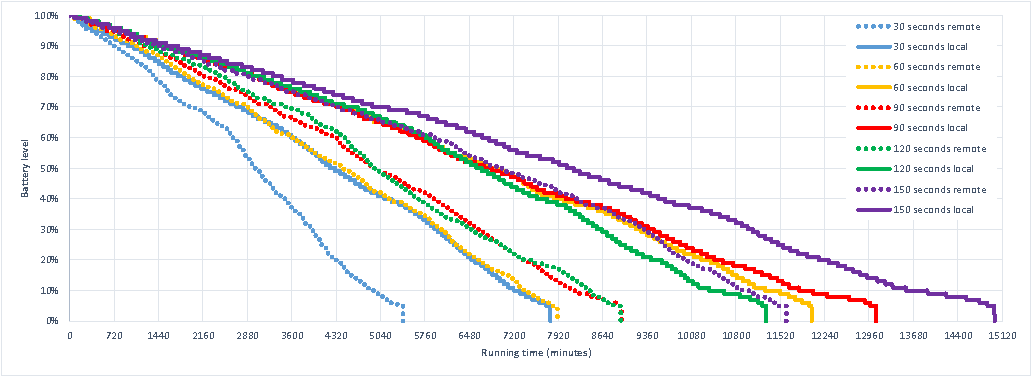
\includegraphics[width=\columnwidth]{vectors/plot-energy-performance-r2}
  \caption{Energy performance comparison of on-device vs MCC oriented sample apps using different GPS sampling periods.}
  \label{fig:plot-energy-performance}
\end{figure}
\end{frame}

\begin{frame}{Preliminary results}{Early adaptive sampling implementation}
Recall the cognitive components are implementing and reacting to changes in mobility.
Such changes are detected and learned by the platform.
Although reaction is expressed as in simple policies, the platform now could implement something else.
\end{frame}



\section{Publications}
\begin{frame}{Publications}{}
Two journal articles have been published along the development of thesis work:
\begin{itemize}
  \item Pérez-Torres, R., Torres-Huitzil, C., \& Galeana-Zapién, H. (2016). Power management techniques in smartphone-based mobility sensing systems: A survey. \emph{Pervasive and Mobile Computing}, 1-21. https://doi.org/10/bds7 \cite{Perez-Torres2016}

  \item Pérez-Torres, R., Torres-Huitzil, C., \& Galeana-Zapién, H. (2016). Full On-Device Stay Points Detection in Smartphones for Location-Based Mobile Applications. \emph{Sensors}, 16(10), 1693. https://doi.org/10/brst \cite{Perez-Torres2016b} 
\end{itemize}
\end{frame}

\begin{frame}{Future work}{Specific activities}
{
\small{}
Next are tasks to be performed in short-term towards defining policies to be implemented by the system solution.
\begin{itemize}
  \item Preliminary integral experimentation for studying mobility information generated by cognitive components.
  \item Selection of mobility cases on which platform will be tested.
  \item Prepare and launch experiments using those scenarios, towards detecting anomalies not observed by the platform.
  \item Definition of policies - behaviors that allow platform to identify and react to such cases accordingly.
  \item Build a software library for exploring - interpreting the mobility information collected by platform.
  \item Evaluate, by experimentation, the policies defined for addressing the issues on mobility cases.
  \item Selection of policies with the best time-spatial accuracy metrics.
\end{itemize}
}
\end{frame}


\section{Future work}
\begin{frame}{Detailed schedule}
\begin{table}[]
\centering
\resizebox{0.95\textwidth}{!}{%
\begin{tabular}{clccccccc}
   &                                                                               & 2014 & \multicolumn{3}{c}{2015} & \multicolumn{3}{c}{2016}  \\
   \cline{3-9}
\multicolumn{2}{l}{\small{Work: \markdone~Done, \markonprogress~In progress, \markoff~To be done}} & 3rd & 1st & 2nd & 3rd & 1st & 2nd & 3rd \\
   \toprule
\multicolumn{2}{c}{\textsc{Step I}}                                                &  &  &  &  &  &  &  \\
1  & State-of-art reading                                                          & \markdone & \markdone &  &  &  &  &  \\
2  & State-of-art works categorization                                             &  & \markdone & \markdone  &  &  &  &  \\
3  & Documentation of information found (committee request)                        &  &  & \markdone &  &  &  &  \vspace{1em}\\

\multicolumn{2}{c}{\textsc{Step II}}                                               &  &  &  &  &  &  &  \\
4  & \makecell[l]{Development of a mobile app for accelerometer and location \\data collection}    &  &  & \markdone & \markdone  &  &  &  \\
5  & Analysis of data                                                              &  &  &  & \markdone  &  &  &  \\
6  & Formal definition of mobility pattern                                         &  &  &  & \markdone &  &  &  \\
7  & Selection of mobility patterns                                                &  &  &  & \markdone & \markdone &  &  \vspace{1em}\\

\multicolumn{2}{c}{\textsc{Step III}}                                              &  &  &  &  &  &  &  \\
8  & Research on classification algorithms for mobility patterns                   &  &  &  & \markdone & \markdone &  &  \\
9  & Definition of metrics for evaluating algorithms                               &  &  &  &  & \markdone &  &  \\
10 & Implementation of algorithms in mobile platform                               &  &  &  &  & \markdone & \markdone  &  \\
11 & Selection of best algorithms according to metrics                             &  &  &  &  &  & \markdone &  \vspace{1em}\\

\multicolumn{2}{c}{\textsc{Step IV}}                                               &  &  &  &  &  &  &  \\
12 & Definition and modeling of parameters needed by the PIE                       &  &  &  & \markdone & \markdone & \markdone & \markdone \\
13 & Building of the PIE                                                           &  &  &  & \markdone & \markdone & \markdone & \markdone \\
\bottomrule
\end{tabular}%
}
\caption{Schedule of activities (each column represents a four months period)}
\label{tbl:schedule-part-one}
\end{table}
\end{frame}

\begin{frame}{Detailed schedule}
\begin{table}[]
\centering
\resizebox{0.95\textwidth}{!}{%
\begin{tabular}{clccccccc}
   &                                                                               & \multicolumn{3}{c}{2016} & \multicolumn{3}{c}{2017} & 2018 \\
   \cline{3-9}
\multicolumn{2}{l}{\small{Work: \markdone~Done, \markonprogress~In progress, \markoff~To be done}}   & 1st & 2nd & 3rd & 1st & 2nd & 3rd & 1st \\
   \toprule
\multicolumn{2}{c}{\textsc{Step V}}                                                &  &  &  &  &  &  & \\
14  & Formal definition of policy                                                  &  &  & \markdone &  &  &  & \\
15  & \makecell[l]{Research and evaluation of techniques for\\generation and adaption of policies}&  &  & \markonprogress & \markonprogress  &  &  & \\
16  & Design and execution of experiments applied to use cases                     &  &  & \markonprogress & \markonprogress  &  &  & \\
17  & Selection of policies                                                        &  &  &  & \markonprogress  &  &  & \vspace{1em} \\

\multicolumn{2}{c}{\textsc{Step VI}}                                               &  &  &  &  &  &  & \\
18  & Definition and modeling of PGE parameters                                    &  &  &  &  & \markonprogress  &  & \\
19  & Building of the PGE                                                          &  &  &  &  & \markonprogress  &  & \vspace{1em} \\

\multicolumn{2}{c}{\textsc{Step VII}}                                               &  &  &  &  &  &  & \\
20  & Analysis of components into software abstractions                             &  &  &  &  & \markdone  &  & \\
21  & Research on Android API for specialized components                            &  &  &  &  & \markdone  &  & \\
22  & Development of middleware                                                     &  &  &  &  & \markonprogress  &  & \vspace{1em}\\

\multicolumn{2}{c}{\textsc{Step VIII}}                                              &  &  &  &  &  &  & \\
23  & \makecell[l]{Definition of experiments aimed at accuracy\\and energy consumption metrics}    &  &  &  &  &  & \markoff & \\
24  & Development of experimental sample mobile apps                                &  &  &  &  &  & \markoff & \\
25  & Experiments execution                                                         &  &  &  &  &  & \markoff & \markoff  \\
26  & Final results analysis                                                              &  &  &  &  &  &  & \markoff \\
\bottomrule
\end{tabular}%
}
\caption{Schedule of activities (each column represents a four months period)}
\label{tbl:schedule-part-two}
\end{table}
\end{frame}

\begin{frame}{Detailed schedule}
\begin{table}
\centering
\resizebox{\textwidth}{!}{%
\begin{tabular}{clcccccccccccc}
   &                                                                               & 2014 & \multicolumn{3}{c}{2015} & \multicolumn{3}{c}{2016} & \multicolumn{3}{c}{2017} & \multicolumn{2}{c}{2018} \\
   \cline{3-14}
 \multicolumn{2}{l}{\small{Work: \markdone~Done, \markonprogress~In progress, \markoff~To be done}} & 3rd & 1st & 2nd & 3rd & 1st & 2nd & 3rd & 1st & 2nd & 3rd & 1st & 2nd\\
   \toprule
\multicolumn{2}{c}{\textsc{Required tasks}}                                        &  &  &  &  &  &  &  &  &  &  &  & \\
A   & Related courses                                                              & \markdone  & \markdone  & \markdone &  &  &  &  &  &  &  &  & \\
B   & Research articles submission                                                 &  &  &  & \markdone &  & \markdone &  &  &  &  & \markoff & \\
C   & Predoctoral exam preparation                                                 &  &  &  &  &  &  &  &  & \markoff &  &  & \\
D   & Thesis writing                                                               & \markdone  &  &  & \markdone &  &  & \markonprogress &  &  & \markoff & \markoff & \markoff \\

\bottomrule
\end{tabular}%
}
\caption{Schedule of required activities}
\label{tbl:schedule-required-activities}
\end{table}
\end{frame}

\section{Conclusions}
\begin{frame}{Conclusions}{}
As conclusions, the current talk has been provided:
\begin{itemize}
  \item lualatex
\end{itemize}
\end{frame}

{\aauwavesbg
\begin{frame}[plain,noframenumbering]
  \finalpage{
    Thank you for your attention!
  }
  { \tiny
    \epigraph{\tiny We make our world significant by the courage of our questions and by the depth of our answers.}{\tiny \textit{Carl Sagan}}
  }
\end{frame}}

\begin{frame}[allowframebreaks]
        \frametitle{References}
%\bibliographystyle{plain}
{
\tiny{}
\bibliographystyle{unsrt}
\bibliography{../../../../../resources/references/library}
}
\end{frame}


\begin{frame}[t]\frametitle{State-of-art solutions}
\begin{table}
    \centering
    \scriptsize{}
    \resizebox{\textwidth}{!} { 
    \begin{tabular}{C{0.11\textwidth}C{0.2\textwidth}C{0.17\textwidth}C{0.15\textwidth}C{0.09\textwidth}C{0.05\textwidth}C{0.05\textwidth}C{0.05\textwidth}}
    \toprule
    \textbf{Name} & \textbf{Variants} & \textbf{Machine learning technique} & \textbf{Sensors involved} & \textbf{Complexity} & \textbf{OL} & \textbf{OO} & \textbf{US} \\
    \midrule

    
    % Category Basic context policy (short time window)
    \emph{G-Sense}      \cite{Perez2010} & User behavior learning (DC) & SDR & GPS & low \\

    \cmidrule(l){1-8}
    Perez-Torres           \cite{Perez-Torres2012} & User behavior learning (DC) & SDR & GPS & low \\

    \cmidrule(l){1-8}
    \emph{SenseLess}    \cite{Abdesslem2009} & User behavior learning (DC), Sensor replacement (CR, DR) & SDR & WPS, GPS, ACC & low \\
    
    \cmidrule(l){1-8}
    \emph{SensTrack}    \cite{Zhang2013} & User behavior learning (DC), Sensor replacement (CR, DR) & SDR & ACC, orientation sensor, GPS, WPS & low \\
    
    \cmidrule(l){1-8}
    Man and Ngai           \cite{Man2014} & User behavior learning (DC, VI), Sensor replacement (CR) & SDR & ACC, magnetic field sensor, GPS & low \\

    \cmidrule(l){1-8}
    \emph{EnLoc}        \cite{Constandache2009} & User behavior learning (DC, VI), Sensor replacement (DR) & SDR, Mobility Tree & WPS, GPS, cellular ID & medium & & \checkmark \\
    
    \cmidrule(l){1-8}
    \emph{EnTracked}    \cite{Kjaergaard2009} & User behavior learning (DC), Sensor replacement (CR) & SDR & ACC, GPS & medium & & \checkmark \\
    \bottomrule
    \end{tabular}
    }
    \protect\caption{Pure software solutions. (OL: Online Learning from user data, OO: Optimization Oriented solution, US: User State context insight)\label{tab:works-software-approach-1}}
\end{table}
\end{frame}

\begin{frame}[t]\frametitle{State-of-art solutions}
\begin{table}
    \centering
    \scriptsize{}
    \resizebox{\textwidth}{!} { 
    \begin{tabular}{C{0.11\textwidth}C{0.2\textwidth}C{0.17\textwidth}C{0.15\textwidth}C{0.09\textwidth}C{0.05\textwidth}C{0.05\textwidth}C{0.05\textwidth}}
    \toprule
    \textbf{Name} & \textbf{Variants} & \textbf{Machine learning technique} & \textbf{Sensors involved} & \textbf{Complexity} & \textbf{OL} & \textbf{OO} & \textbf{US} \\
    \midrule

    % Category Medium context-aware policy
    Alvarez, Morillo           \cite{AlvarezDeLaConcepcion2014,Morillo2015} & --- & Ameva algorithm & ACC & medium \\
    
    \cmidrule(l){1-8}
    Mazilu           \cite{Mazilu2013} & Sensor replacement (CR) & DT & Temperature, humidity, pressure & medium \\
    % Not given           \cite{Mazilu2013} & Sensor replacement (CR) & DT (C4.5) & Temperature, humidity, pressure & medium \\

    \cmidrule(l){1-8}
    Srinivasan           \cite{Srinivasan2012} & User behavior learning (DC) & DT & ACC & medium \\
    
    \cmidrule(l){1-8}
    Khalifa           \cite{Khalifa2015} & Sensor replacement (CR) & KNN & Model of ACC-based harvesting device & medium \\
    \bottomrule
    \end{tabular}
    }
    \protect\caption{Pure software solutions. (OL: Online Learning from user data, OO: Optimization Oriented solution, US: User State context insight)\label{tab:works-software-approach-2}}
\end{table}
\end{frame}


\begin{frame}[t]\frametitle{State-of-art solutions}
\begin{table}
    \centering
    \scriptsize{}
    \resizebox{\textwidth}{!} { 
    \begin{tabular}{C{0.11\textwidth}C{0.2\textwidth}C{0.17\textwidth}C{0.15\textwidth}C{0.09\textwidth}C{0.05\textwidth}C{0.05\textwidth}C{0.05\textwidth}}
    \toprule
    \textbf{Name} & \textbf{Variants} & \textbf{Machine learning technique} & \textbf{Sensors involved} & \textbf{Complexity} & \textbf{OL} & \textbf{OO} & \textbf{US} \\
    \midrule

    % Category Long time window
    \emph{SensLoc}         \cite{Kim2010} & User behavior learning (DC, RD), Sensor replacement (CR) & SDR & Wi-Fi fingerprinting, GPS, ACC & medium & \checkmark & \\
    
    \cmidrule(l){1-8}
    \emph{CAPS}         \cite{Paek2011} & User behavior learning (DC, RD), Sensor replacement (CR) & SDR & GPS, cellular ID & medium & \checkmark \\
    % SDR (Smith-Waterman algorithm) CR because location is processed alternatively with this algorithm

    \cmidrule(l){1-8}
    \emph{RAPS}         \cite{Paek2010} & User behavior learning (DC, RD), Sensor replacement (CR, DR) & SDR & WPS, GPS, ACC, Bluetooth, cellular ID & medium & \checkmark \\
    
    % In-between Category Optimization + long time window
    \cmidrule(l){1-8}
    \emph{A-Loc}        \cite{Lin2010} & User behavior learning (DC, RD), Sensor replacement (CR, DR) & HMM, Bayesian estimation framework & GPS, WPS, Bluetooth, cellular ID & medium & \checkmark & \checkmark  \\
    
    \cmidrule(l){1-8}
    \emph{SmartDC}      \cite{Chon2011} & User behavior learning (DC, RD), Sensor replacement (CR, DR) & HMM and LZ predictor & GPS, WPS, Wi-Fi and cellular ID fingerprinting & medium & \checkmark & \checkmark \\
    
    \bottomrule
    \end{tabular}
    }
    \protect\caption{Pure software solutions. (OL: Online Learning from user data, OO: Optimization Oriented solution, US: User State context insight)\label{tab:works-software-approach-3}}
\end{table}
\end{frame}

\begin{frame}[t]\frametitle{State-of-art solutions}
\begin{table}
    \centering
    \scriptsize{}
    \resizebox{\textwidth}{!} { 
    \begin{tabular}{C{0.11\textwidth}C{0.2\textwidth}C{0.17\textwidth}C{0.15\textwidth}C{0.09\textwidth}C{0.05\textwidth}C{0.05\textwidth}C{0.05\textwidth}}
    \toprule
    \textbf{Name} & \textbf{Variants} & \textbf{Machine learning technique} & \textbf{Sensors involved} & \textbf{Complexity} & \textbf{OL} & \textbf{OO} & \textbf{US} \\
    \midrule

    % Category Full context-aware policy
    \emph{Jigsaw}       \cite{Lu2010} & User behavior learning (DC), Sensor replacement (CR) & Microphone: NB with Gaussian Mixture Model (GMM). ACC: DT. GPS: MDP. & ACC, Microphone, GPS & high & & \checkmark & \checkmark \\
    
    \cmidrule(l){1-8}
    Donohoo           \cite{Donohoo2014} & User behavior learning (DC) & Several. KNN and NN selected as best. & ACC, GPS, WPS, cellular ID, light, device data, mobile app requirements & high & & & \checkmark \\

    \cmidrule(l){1-8}
    \emph{EEMSS}        \cite{Wang2009} & User behavior learning (DC), Sensor replacement (CR, DR) & GPS and ACC: SDR. \newline Microphone: SSCH algorithm. & ACC, microphone, GPS & high & & & \checkmark \\

    \cmidrule(l){1-8}
    \emph{iLoc}         \cite{MaY2009} & User behavior learning (RD), Sensor replacement (CR) & HMM & Wi-Fi \& GSM fingerprinting & high & \checkmark & & \checkmark  \\
    
    \cmidrule(l){1-8}
    Yurur           \cite{Yurur2014} & User behavior learning (DC, RD) & HMM & ACC & high & \checkmark & & \checkmark \\
    
    \cmidrule(l){1-8}
    \emph{FreeTrack}    \cite{Chon2014} & User behavior learning (DC, RD), Sensor replacement (CR, DR) & HMM & GPS, Wi-Fi, cellular ID, battery status & high & \checkmark & & \checkmark \\
    
    \bottomrule
    \end{tabular}
    }
    \protect\caption{Pure software solutions. (OL: Online Learning from user data, OO: Optimization Oriented solution, US: User State context insight)\label{tab:works-software-approach-4}}
\end{table}
\end{frame}

\begin{frame}{Additional experiments results}{Accuracy evaluation of detected stay points}
\begin{table}
\centering
\caption{Spatial and time accuracy observed in results of first experiment (SP = stay point).}
\label{tbl:experiment-1-spatial-time-accuracy}
\resizebox{0.7\textwidth}{!}{%
\begin{tabular}{@{}ccccc@{}}
\toprule
\textbf{\begin{tabular}[c]{@{}c@{}}Sampling\\ period \\ (seconds)\end{tabular}} & \textbf{\begin{tabular}[c]{@{}c@{}}Event-driven\\ algorithm\end{tabular}} & \textbf{\begin{tabular}[c]{@{}c@{}}Detected\\ SP's\end{tabular}} & \textbf{\begin{tabular}[c]{@{}c@{}}Average SP stay \\  time difference\\ (seconds)\end{tabular}} & \textbf{\begin{tabular}[c]{@{}c@{}}Average SP\\ distance difference \\  (meters)\end{tabular}} \\ \midrule
\multirow{2}{*}{30} & Buffered & 16 (out of 19)$^\dagger$ & 64.13 & 13.35 \\
 & Sigma & 19 (out of 19) & 68.78 & 16.01 \\
 \cmidrule{2-5}

\multirow{2}{*}{60} & Buffered & 29 (out of 29) & 98.24 & 14.97 \\
 & Sigma & 21 (out of 29)$^\dagger$ & 82.35 & 19.42 \\
 \cmidrule{2-5}

\multirow{2}{*}{90} & Buffered & 20 (out of 20) & 104.95 & 20.6 \\
 & Sigma & 20 (out of 20) & 211.68 & 20.68 \\
 \cmidrule{2-5}

\multirow{2}{*}{120} & Buffered & 19 (out of 21)$^\dagger$ & 63.7 & 35.56 \\
 & Sigma & 21 (out of 21) & 59.7 & 34.05 \\
 \cmidrule{2-5}

\multirow{2}{*}{150} & Buffered & 24 (out of 29)$^\dagger$ & 116.4 & 59.11 \\
 & Sigma & 28 (out of 29)$^\ddagger$ & 115.6 & 50.81 \\

\bottomrule
\end{tabular}%
}

{\scriptsize $\dagger$ Due to battery depletion, $^\ddagger$ Actual SP miss}

\end{table}
\end{frame}

\end{document}
